 \section*{Methods}
 \label{methods}

%Methods each state has feature vector. Problem: describe set of states satisfying a given condition: this could be one feature or a combination of features 
%Clause: and of some features 
%Expression which is a sum and difference of clauses 
%MDL criterion 
%Minimization is np hard
%IP for finding best description 

\subsection*{Notation and Problem Formulation}

Let $U$ denote a set of elements of interest; we focus on regions, primarily states
in the US, though our abstraction easily extends to other notions of regions,
and other kinds of objects. We will use elements and states synonymously.
There are different kinds of features associated with each state;
examples of features that can be used for the Influenza data from CDC are:
\begin{itemize}
\item
Location (e.g., Mid-Atlantic, Southwest)
\item
Activity level (e.g., high, moderate and low) in the $t$th week before the current one 
\item
Geographical spread (e.g., widespread, local) in the $t$th week before the current one
\item
Whether the number of infections has crossed a threshold
\item
Whether the peak has been reached
\item
Similarity with past season.
\end{itemize}

All these features other than the first one (location) are epidemic specific, and
are computed by CDC using specific definitions. These features capture the spatial, temporal,
and severity aspects of the reported cases. We use CDC reports, e.g., \cite{cdc:surveillance-report-feb10}, for data on
these features. We combine the data for
multiple weeks (e.g., for the activity level in the $t$th week before the
current one), and multiple seasons (e.g., for the similarity with past seasons) for our study.
In general, these values are real numbers, e.g., the similarity with a past season
can be a correlation metric.  In this paper, we will focus on binary features
(e.g., high/low activity level, which is already available in the data from CDC).
The non-binary setting can be mapped to a binary setting, through discretization
of the weights.

The input data can be viewed as a matrix $D_{n\times m}$, with rows corresponding
to the states, and columns corresponding to features.
We denote the $j$th feature as the $j$th column, with $D_{ij}=1$ if state $i$ has
that feature. For instance, suppose the $j$th feature indicates a ``mid-atlantic state''.
Then, $D_{ij}=1$ for states $i$ corresponding to NY and PA, but is 0 for CA. 
For activity levels, we have separate features for the past weeks. 
In addition, all the rows are also used as features (i.e., columns). The reason for this will be made clear in the description below. Table \ref{sampledata} shows part of an example of such a matrix $D$, and will be
used as a running example to explain all our definitions and problem formulation.

\noindent
\begin{table}[ht!]
\begin{tiny}
\begin{center}
\begin{tabular}{| p{0.5cm}| p{1.0cm}| p{1.0cm}| p{1cm}| p{1cm}| p{1.0cm}| p{1.0cm}|p{0.5cm}|p{0.5cm}|p{0.5cm}|p{0.5cm}|p{0.5cm}|p{0.5cm}|} \hline
& (South East) & (Mid-Atlantic) & (Was1-high) & (Was1-low) & (Was2-low) & (Was52-high) & ($e_1$) & ($e_2$) & ($e_3$) & ($e_4$) & ($e_5$) & ($e_6$)\\ 
& $f_1$& $f_2$ & $f_3$  & $f_4$ & $f_5$ & $f_6$ & $f_7$ & $f_8$ & $f_ 9$ & $f_{10}$ & $f_{11}$ & $f_{12}$ \\ \hline
$e_1$ & 1 & 1 & 1 & 0 & 0 & 1 & 1 & 0 & 0 & 0 & 0 & 0\\ \hline
$e_2$ & 0 & 0 & 0 & 1 & 0 & 1 & 0 & 1 & 0 & 0 & 0 & 0\\ \hline
$e_3$ & 0 & 0 & 0 & 0 & 1 & 0 & 0 & 0 & 1 & 0 & 0 & 0\\ \hline
$e_4$ & 1 & 1 & 1 & 0 & 1 & 0 & 0 & 0 & 0 & 1 & 0 & 0\\ \hline 
$e_5$ & 1 & 1 & 0 & 0 & 1 & 1 & 0 & 0 & 0 & 0 & 1 & 0\\ \hline
$e_6$ & 0 & 0 & 1 & 0 & 0 & 1 & 0 & 0 & 0 & 0 & 0 & 1\\
\hline
\end{tabular}
\caption{
Sample input, represented as a matrix $D$ of dimensions $6\times 12$. The rows (corresponding to states) are elements of $U$, and the first six columns are features. The next six columns are added for computational reasons.
%%The set $U=\{e_1,\ldots,e_6\}$ represents the set of elements.
%%The columns $f_1,\ldots,f_6$ represent the original features for
%%each element $e_i$. In this example each feature is associated with
%%some characteristic of the incidence data, e.g., $f_1$ corresponds to
%%``South East''.
%%The row names will also be considered as attributes/features in our formulation.
}
\label{sampledata}
\end{center}
\end{tiny}
\end{table}


\noindent
\textbf{Example.}
\begin{table}[ht!]
\begin{small}
\begin{center}
\begin{tabular}{| p{1cm} | p {2.8cm} | p{7.5cm}|}
\hline
\textbf{Term} & \textbf{Definition} & \textbf{Description} \\
\hline 
$U$ & $\{e_1, ..., e_n\}$ & Universe set \\ 
\hline
$T$ & $T \subseteq U$ & Target set \\
\hline
$D_j$ & $\{i: D_{ij}=1\}$ & Set of elements having feature $j$ \\
\hline
$\mathbf{j}^{\ell}$ & $j_1,\ldots,j_k$ & List of features $j_1,\ldots,j_k$ in ${\ell}^{th}$ clause\\
\hline
$S(\mathbf{j}^{\ell})$ & $D_{j_1}\cap \ldots \cap D_{j_k}$ & Set of elements that have all features in list $\mathbf{j}^{\ell}$ \\
\hline
\end{tabular}
\caption{Definitions and notations used in the paper}
\label{notations}
\end{center}
\end{small}
\end{table}
An example of the input data is shown in Table \ref{sampledata}, in the form of
a matrix $D$. It has six rows (corresponding to regions), 
denoted here by $\{e_1, e_2, e_3, e_4, e_5, e_6\}$.
$D$ has twelve columns, denoted here by $\{f_1, f_2, f_3, f_4, f_5, f_6\}$,
in addition to one column for each row. The first six columns
correspond to features, e.g., ``South East'' (which means the region is in
South Eastern US) and ``Was1_high'' (which means the region was high last week).

We start with some definitions needed for 
formalizing this problem. Let $U = \{e_1, ..., e_n\}$ be the universe of elements, in our case, the set of all states. Let $D_j=\{i: D_{ij}=1\}$ denote the set of
elements having feature $j$. Let $S(j_1,\ldots,j_k) = D_{j_1}\cap \ldots \cap D_{j_k}$
denote the set of elements that have features $j_1,\ldots,j_k$; we will refer to
such a set as a conjunctive \emph{clause}.  We will sometimes say that such a clause
$S(j_1,\ldots,j_k)$ has length $k$, meaning that it is formed by the intersection of
$k$ features.  We associate a cost $c(j_1,\ldots,j_k)$ function;
the simplest would be $c(j_1,\ldots,j_k)=\alpha k$ for a constant $\alpha$.

\noindent
\textbf{Example.}	
Let $U = \{e_1, e_2, e_3, e_4, e_5, e_6 \}$. In the matrix D in Table \ref{sampledata},
$D_2 = \{e_1, e_4, e_5\}$ and $D_5 = \{e_3, e_4, e_5\}$ are
examples of sets having features $f_2$ and $f_5$, respectively.
Then, $S(2, 5)$ is a clause, which represents the set
$S(2, 5) = D_2 \cap D_5 = \{e_4, e_5\}$. Note that the column $D_7=\{e_1\}$
is also a clause, represented by $S(7)$.

%%The main problem we consider here is to construct descriptions for
%%a subset $T\subseteq U$ of elements. Our overall goal is to ensure that the
%%descriptions are intuitive and explainable, and we use the 
%%\emph{Minimum Description Length} (MDL) Principle, that forms the basis of many
%%machine learning methods to find such descriptions; we refer to \cite{grunwald:07:book}
%%for details on this topic. 
%%Specifically, we find a \emph{succinct} representation of the set $T$ of elements,
%%in terms of combinations of different features.
%%For instance, suppose the set of states which are currently high are precisely
%%those in the East and South.
%%These could be described in two alternate ways:
%%(a) by just listing all the states (e.g., VA, NC, MD, etc.) or,
%%(b) as just Eastern and Southern states. The latter is preferred because of its succinctness.
%%

Given a target set $T\subseteq U$,
we consider expressions of $T$ in terms of unions and differences of such clauses,
having the following form
\[
T = \bigcup_{\ell=1}^r S(j^{\ell}_1,\ldots,j^{\ell}_{k_{\ell}}) - 
 \bigcup_{\ell=r+1}^s S(j^{\ell}_1,\ldots,j^{\ell}_{k_{\ell}}),
\]
with an associated cost of
\[
\sum_{\ell=1}^r \alpha k_{\ell} + \sum_{\ell=r+1}^s \beta k_{\ell},
\]
where $\alpha$ and $\beta$ are the constant parameters associated with positive
and negative clauses.
The clauses $S(j^{\ell}_1,\ldots,j^{\ell}_{k_{\ell}})$ corresponding to $\ell=1,\ldots,r$
will be viewed as ``positive'' clauses, and $\alpha$ is the cost for each such clause.
The clauses corresponding to $\ell=r+1,\ldots,s$ are referred to as ``negative'' clauses, 
and describe elements which need to be removed from the set of positive clauses, in order to
exactly cover the elements of $T$; the cost parameter corresponding to the negative
clauses is $\beta$.  
For succinctness, we use $\mathbf{j}^{\ell}=(j^{\ell}_1,\ldots,j^{\ell}_{k_{\ell}})$ to denote
such a tuple, and $S(\mathbf{j}^{\ell}) = S(j^{\ell}_1,\ldots,j^{\ell}_{k_{\ell}})$ as the
corresponding clause. We use $\numf(\mathbf{j}^{\ell})=k_{\ell}$ to denote the
number of features involved in such a clause. Then, the representation for $T$
can be written as 
\[
T = \bigcup_{\ell=1}^r S(\mathbf{j}^{\ell}) - \bigcup_{\ell=r+1}^s S(\mathbf{j}^{\ell}),
\]
with an associated cost of 
\[
\sum_{\ell=1}^r \alpha\cdot \numf(\mathbf{j}^{\ell}) + \sum_{\ell=r+1}^s \beta\cdot \numf(\mathbf{j}^{\ell}).
\]
Finally, we use $\mathcal{C}^k=\{\mathbf{j}=(j_1,\ldots,j_{k'}): k'\leq k\}$ to denote
the set of all such tuples of length at most $k$;
for an element $i$, let $\mathcal{C}^k_i=\{\mathbf{j}=(j_1,\ldots,j_{k'}): k'\leq k, i\in S(\mathbf{j})\}$
denote the set of tuples such that the corresponding clauses contain $i$. 

\noindent
\textbf{Example.} 
We continue our example from Table \ref{sampledata}. An example of a target
set $T$ is the set of regions that have feature $f_1$, i.e, $T = \{e_1, e_4, e_5\}$.
$T$ can be expressed as combinations of different kinds of clauses.
For instance, $T=S(7)\cup S(10) \cup S(11)$. This representation has cost $3\alpha$.
Note that $D_2=D_1=T$, so $T$ can also be expressed simply as $T=S(2)$; this
has cost $\alpha$.
Finally, We can represent $T$ the target set as unions and differences of clause as
$T = S(2, 5) \cup S(3, 6) - S(3,4,6)$, since
$S(2, 5) = D_2\cap D_5=\{e_4, e_5\}$
$S(3, 6) = D_3 \cap D_6 \{e_1, e_6\}$,
$S(3, 4, 6) = D_3 \cap D_4 \cap D_6 = \{e_6\}$.
However, this representation has cost $2\alpha + 2\alpha + 3\beta=4\alpha+3\beta$.

\noindent
\textbf{Problem formulation: the \mindesc{} problem.} 
Given a subset $T\subseteq U$ (referred to as a ``target'' set),
and a dataset $D$, the \mindesc{}$(T, D)$ problem involves
finding a set of tuples $\mathbf{j}^{1},\ldots,\mathbf{j}^{s}$,
such that
\[
T = \bigcup_{\ell=1}^r S(\mathbf{j}^{\ell}) - \bigcup_{\ell=r+1}^s S(\mathbf{j}^{\ell}),
\]
and the associated cost
$\sum_{\ell=1}^r \alpha\cdot \numf(\mathbf{j}^{\ell}) + \sum_{\ell=r+1}^s \beta\cdot \numf(\mathbf{j}^{\ell})$ is minimized. 
In order to make the descriptions interpretable, we will restrict the sizes of
these clauses, i.e., the number $k_{\ell}$ of columns whose intersection is allowed;
here, we will focus on $k_{\ell}\leq 2$, though our approach extends to any $k$.

Our main idea for finding patterns of interest is to explore the space of
all target sets, and identify those which have low cost descriptions.
This is motivated by the \emph{Minimum Description Length} (MDL) Principle, that forms the basis of many
machine learning methods to find such descriptions; we refer to \cite{grunwald:07:book}
for details on this topic.
Specifically, we find a \emph{succinct} representation of the set $T$ of elements,
in terms of combinations of different features.
For instance, suppose the set of states which are currently high are precisely
those in the East and South.
These could be described in two alternative ways:
(a) by just listing all the states (e.g., VA, NC, MD, etc.) or,
(b) as just Eastern and Southern states. The latter is preferred because of its succinctness.

Note that for each element in $U$ there is a feature in our data matrix. This is required to be able to represent
any given target set $T$ in terms of unions and differences of clauses.

%The addition of one feature for each row guarantees that every instance of the problem has a feasible solution. Let us assume that this requirement is not enforced. The union of the positive clauses would cover the target set and some more elements. To remove an extra element from this union, a negative clause must pick a set containing this element. We can construct instances that have no set that contains this extra element and is disjoint with $T$.  Then the negative clause has no set to pick to remove the extra element without removing any element of target set from the representation. But with the availability of a singleton set for every element as a feature, the negative clause could just pick the singleton set containing this extra element, therefore guaranteeing the feasibility.

\noindent
\textbf{Example.}	
Continuing our example, let $T = \{e_1, e_3, e_4\}$. Assume that we can only use features $f_1, ..., f_6$ in the clauses to represent $T$ in required form. Then, $S(1) \cup S(5) = \{e_1, e_3, e_4, e_5\} $ (alternatively, $S(2) \cup S(5)$ ) covers all elements of $T$ with just one extra element $e_5$. This element can not be removed by any choice of a negative clause without removing $e_1$. 

\noindent
\textbf{Relaxed descriptions.} 
As discussed in the example in Figure \ref{fig:jan27}, in some cases, the
target set $T$ does not have a small description, but we can find a set $T'$
which is \emph{close} to $T$, and has a smaller description than $T$.
We model this as finding a representation for
a subset $T'$ such that $T'\approx T$, which is formalized as the
\minapproxdesc{} problem:
\begin{quote}
Given a target set $T\subseteq U$, a dataset $D$, and constant parameters
$\alpha, \beta, \gamma$, the \minapproxdesc{}$(T, D)$ problem involves
finding a set of tuples $\mathbf{j}^{1},\ldots,\mathbf{j}^{s}$,
such that
\[
T' = \bigcup_{\ell=1}^r S(\mathbf{j}^{\ell}) - \bigcup_{\ell=r+1}^s S(\mathbf{j}^{\ell}),
\]
$|\{i: i\in T\setminus T'\cup T'\setminus T\}| \leq\gamma |T|$,
and the associated cost
$\sum_{\ell=1}^r \alpha\cdot \numf(\mathbf{j}^{\ell}) + \sum_{\ell=r+1}^s \beta\cdot \numf(\mathbf{j}^{\ell})$ is minimized. 
We refer to $\alpha, \beta, \gamma$ as the parameters associated with the
relaxed version.
\end{quote}

In other words, the \minapproxdesc{} problem finds a representation for a subset $T'$
that is ``close'' to $T$.

\noindent
\textbf{Finding low cost descriptions for a target set $T$: solving the \mindesc{}
and \minapproxdesc{} problems.}
The \mindesc{} and \minapproxdesc{} problems are both
NP-complete, even when $k_{\ell}= 1$, which corresponds to the \emph{set cover}
problem (we refer to \cite{GareyJohnson} for discussion on this topic). 
Here, we use an integer programming
approach described in the Appendix,
which is able to scale well for the problems of interest in epidemic analysis. 
We use the Gurobi optimization software \cite{gurobi}
to solve the resulting Integer program. The size of instances encountered results in programs 
that can be solved very efficiently. So we expect our method will scale to much larger datasets easily. 


\noindent
\textbf{Overall workflow: finding ``interesting'' patterns by
exploring different potential target sets.}
Our integer programming approach gives a low cost description for any given target
set $T$. As mentioned earlier, from the MDL principle, a set $T$ is likely
to be an interesting pattern if it has a low cost representation---we
refer to this as a ``succinct description''.
Motivated by this idea, we discover interesting patterns by exploring
many potential target sets, and ranking them based on their description cost,
as we describe below.
\begin{itemize}
\item
We consider clauses $S(\mathbf{j})$ with $\numf(\mathbf{j})\leq k$, i.e.,
all possible clauses of length at most $k$, as potential target sets.
Solve the \mindesc{} and \minapproxdesc{} problems for a target set $T=S(\mathbf{j})$;
note that we will only consider representations from the set
$\mathcal{C}^k-\mathbf{j}$ for such a clause $S(\mathbf{j})$.
\item
The potential target sets are partitioned into the following classes:
\begin{itemize}
\item
Specific features: these are individual columns $D_j$, e.g., the set of states
with a ``high activity level'', ``moderate activity level'', etc. These correspond
to the kinds of descriptions in CDC reports, as in \cite{cdc:surveillance-report-feb10}.
\item
Stable trends: these correspond to sets of features which are stable over time, e.g., high activity level for the past three weeks.
\item
Temporal changes: those showing changes in features over a time period, e.g.
low activity in one week and high in the next.
\end{itemize}
\item
Within each class above, the potential target sets are ordered based on the
description cost, computed using the integer programming approach.
We consider both the exact and relaxed representations, and retain
the relaxed representation if its cost is much less.
\end{itemize}

\begin{figure}
\centering
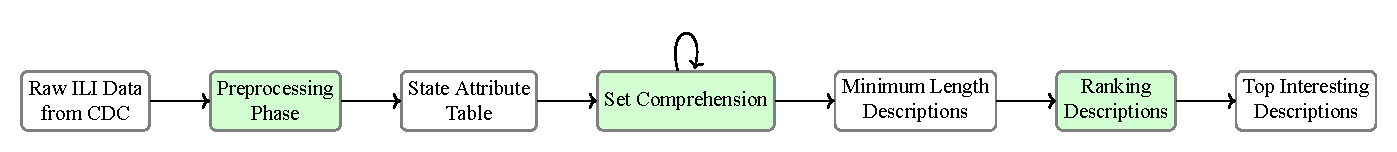
\includegraphics[width=0.95\linewidth]{./figures/epi-summary-pipeline/main.pdf}
\caption{Overview of steps, to generate succinct description of the level of
influenza like illnesses (ILI) in different states of USA.
The process begins with collecting raw ILI data from CDC website,
followed by the creation of a state attribute table ---
a domain-specific version of the transaction-item matrix $D$ --- for a given weekend.
We iterate over a space of all potential target sets, and solve the
\minapproxdesc{} problem to compute a representation. These are then ranked based
on their interestingness score.
%The minimum description length (MDL) inspired summarization technique
%is applied on the state attribute table to generate the succinct descriptions.
}
\label{fig:epi-summary-pipeline}
\end{figure}

Figure~\ref{fig:epi-summary-pipeline} shows an overview of our methodology. 

In the results section, we present some descriptions generated by our algorithm for a particular target set, followed by a discussion on effects of the parameters. Finally, we present the utility of these methods in automatically identifying certain patterns in the data. 
